\documentclass[10pt,twocolumn,letterpaper]{article}

\usepackage{cvpr}
\usepackage{times}
\usepackage{epsfig}
\usepackage{graphicx}
\usepackage{amsmath}
\usepackage{amssymb}

% Include other packages here, before hyperref.

% If you comment hyperref and then uncomment it, you should delete
% egpaper.aux before re-running latex.  (Or just hit 'q' on the first latex
% run, let it finish, and you should be clear).
\usepackage[breaklinks=true,bookmarks=false]{hyperref}

\cvprfinalcopy % *** Uncomment this line for the final submission

\def\cvprPaperID{****} % *** Enter the CVPR Paper ID here
\def\httilde{\mbox{\tt\raisebox{-.5ex}{\symbol{126}}}}

% Pages are numbered in submission mode, and unnumbered in camera-ready
%\ifcvprfinal\pagestyle{empty}\fi
\setcounter{page}{4321}
\begin{document}
	
	%%%%%%%%% TITLE
	\title{A Review of Metric Learning Methods}
	
	\author{First Author\\
		Institution1\\
		Institution1 address\\
		{\tt\small firstauthor@i1.org}
		% For a paper whose authors are all at the same institution,
		% omit the following lines up until the closing ``}''.
		% Additional authors and addresses can be added with ``\and'',
		% just like the second author.
		% To save space, use either the email address or home page, not both
		\and
		Second Author\\
		Institution2\\
		First line of institution2 address\\
		{\tt\small secondauthor@i2.org}
	}
	
	\maketitle
	%\thispagestyle{empty}
	
	%%%%%%%%% ABSTRACT
	\begin{abstract}
		Metric learning is the task of learning a distance function on pair of objects. We review three metric learning methods based on deep learning, including Siamese Network, Triplet Network and n-Tuple Network framework. These frameworks output low dimensional embedding for input data, on which we may use Euclidean distance as the distance function. These frameworks all include a set of neural networks sharing the same structure and parameters and a loss function combining the outputs of the networks. In this work, we wrote a wrapper class for the network to hide the low-level implementation, and focus on the design of the high-level frameworks and loss functions. In our experiment on MNIST dataset and a classic network structure, Siamese Network has a mediocre performance while Triplet Network produces better embeddings. We are not able to make the original n-Tuple Network work. However, we have tested a few modified versions of it, which keep the framework unchanged but use different loss functions.
	\end{abstract}
	
	%%%%%%%%% BODY TEXT
	\section{Introduction}
	Metric learning is the task of learning a distance function on pair of objects. The most trivial definition of distance of two instances (which can be two images, two sequences, etc.) is the Euclidean distance. However, Euclidean distance may not be a good indicator for specialized tasks, because it cannot represent the intrinsic structure of the data. Theoretically, many high dimensional datasets can be viewed as low dimensional manifold embedded in a high dimensional space, where Euclidean distance cannot capture the manifold.
	
	To solve this problem, many Metric learning algorithms are invented. The classical ones include Isomap, Locally Linear Embedding (LLE), Stochastic Neighbor Embedding, etc. These methods are all unsupervised methods. In the deep learning area, LeCun ??? introduces Siamese Network, which can be viewed as a framework including two neural networks of the same structure and sharing the same parameters and a loss function defines on the two outputs and the labels of the two inputs. Commonly, the loss function call for a small distance of the outputs when the two inputs are of the same label and vice versa. Elad Hoffer and Nir Ailon have invented Triplet Network ???, which is an extension of Siamese Network, but includes three networks. The Triplet Network processes two instances from one class and one instance from another class at the same time. ??? n-Tuple Network further generalize the idea of Triplet Network, where two instances from one class and multiple instances from the other classes are used at one time.
	
	We use two laptops to perform the experiments. One of them is equipped with Intel Core i7-5700HQ and NVidia 960M GPU. Another one has Intel Core i7-6500U and 
	NVidia 940M GPU.

	In section \ref{sec:mech} we show the mechanisms of the aforementioned deep learning methods in detail. Some important details about implementation is shown in section \ref{sec:Impl}. We show our experiments and results in \ref{sec:Res}. We further discuss the phenomena shown in the experiments in section \ref{sec:Disc}.
	
	\section{Mechanisms \label{sec:mech}}
		\subsection{Siamese Network}
			Siamese Network is a framework for metric learning. It contains two parts, the twin networks (In fact its name ``Siamese'' is related to twin) and the loss function. The structure of the framework is shown in figure ???. Each one of the twin networks takes one instance from the dataset, denoted as $x_1$ and $x_2$, and output the result $y_1 = Net(x_1)$ and $y_2 = Net(x_2)$ respectively. The loss function is defined as follows. \footnote{Expressions are slightly different from the original paper to keep consistent through our article.}
			\begin{equation}
				Loss = (1-S)L_S(\lvert y_1 - y_2 \rvert) + S L_D(\lvert y_1 - y_2 \rvert)
			\end{equation}
			where $L_S(\bullet)$ and $L_D(\bullet)$ stands for loss functions for similarity and dissimilarity respectively. When $x_1$ and $x_2$ are in the same class (or is similar on some perspective), label $S$ is set to be $1$, and the loss is caused by dissimilarity. When $x_1$ and $x_2$ are not in the same class, $Y$ is set to $0$ and gives a penalty on similarity. The formal definitions of the functions are as follows.

			\begin{equation}
				L_S = \frac{1}{2}\lVert y_1 - y_2 \rVert^2
			\end{equation}
			\begin{equation}
				L_D = \frac{1}{2}\{max(0, m-\lVert y_1-y_2\rVert)\}^2 \label{eq:negative}
			\end{equation}
			where $m$ is a positive parameter. Generally speaking, $L_D$ treats two points whose distance is more than $m$ as totally separated and puts no penalty on them.
			
			For a simple analysis, constrative term \ref{eq:negative} can be essential and $L_S$ is convex and can vanish to zero without it.
		\subsection{Triplet Network}
			Triplet Network is a enhanced version of Siamese Network, which processes similar instance and dissimilar instance at the same time. The structure of the framework is shown in figure ???. The loss function is not just the similarity or dissimilarity, but is based on comparison of the similarity of similar instances and dissimilarity of dissimilar instances. The 

		\subsection{(N+1)-tuple Network}
			As seem in the improvement Triplet Network is making, we can sample several negative examples for the training set, 
			$$(x,x^+,x^-_1,x^-_2,\cdots x^-_{N-1})$$
			But generating $M$ batches of samples like this requires lots of computation burden. So instead of generating $M\times(N+1)$ examples and calculate the loss on them, we generate $N$ pairs of images of the same type and distinct pairs of images are of different labels. And the corresponding $(N+1)-$pair loss is given by 
			\begin{equation}
				L(\{x_i,x_i^+\}^N_{i=1})=\frac{1}{N}\log(\sum_{i=1}^N\exp(\sum_{j=1}^Ny^T_iy_j^+-y_i^Ty_i^+))  \label{eq:n-pair}
			\end{equation}
			As observed in equation \ref{eq:n-pair}, if $\sum^N\limits_{i=1}\exp(y^T_iy_j^+-y_i^Ty_i^+)$ is negative then embeddings $\{C\cdot y_i,C\cdot y_i^+\}$ gives a lower loss with any negative constant $C$, thus restrictions on norm of embeddings are needed.\\
			Several attempts have been made on restricting the norm of embeddings. While none of them shows better performance on metric learning. We adopt a solution described in the paper: Adding $L_2-$ norm for training embeddings in the loss function and this should not only constrain resulting embeddings in a reasonable range, but will also enhance convexity of the system.

			\begin{align}
				&L(\{x_i,x_i^+\}^N_{i=1})\notag\\
				=&\frac{1}{N}\log(\sum_{i=1}^N\exp(\sum_{j=1}^Ny^T_iy_j^+-y_i^Ty_i^+))+ \frac{\lambda}{2N} \sum_{i=1}^N(\lVert y_i\rVert^2+ \lVert y^+_i\rVert^2)
			\end{align}
			\begin{figure}[t]

				\begin{center}
				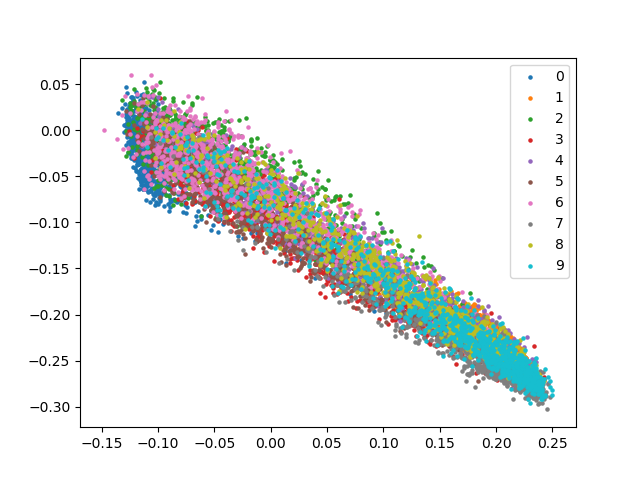
\includegraphics[width=0.5\linewidth]{fig/fig1000}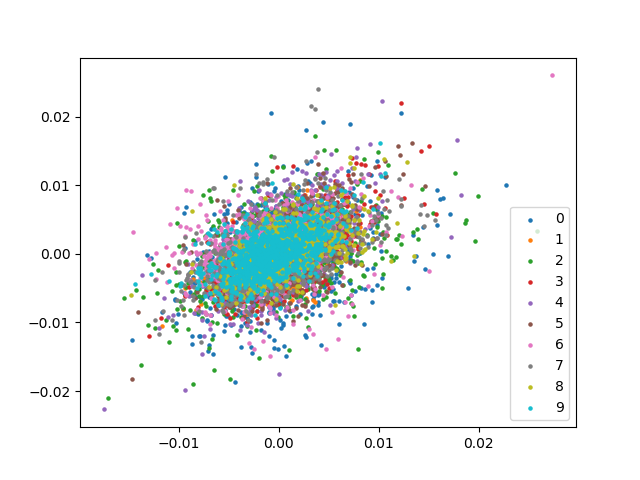
\includegraphics[width=0.5\linewidth]{fig/fig600}
				 \caption{3-pair loss with $\lambda (L_2)^2[\lambda=1.0]$ constraint and constraint $\lambda L_2[\lambda=1.0]$}
				%\fbox{\rule{0pt}{2in} \rule{0.9\linewidth}{0pt}}
   				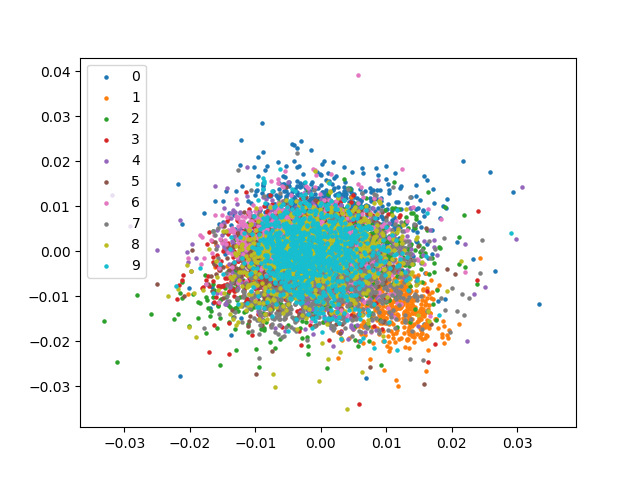
\includegraphics[width=0.9\linewidth]{fig/fig150}
				\end{center}
   \caption{3-pair loss with $\lambda L_2$ constraint and weight $\lambda=0.3$.  We also added negative cutoff $m$ in equation \ref{eq:negative}, this proves improve the training result.}


   Another observation is that while optimizing contrastive loss and triplet loss is approachable for momentum optimizer, we could hardly optimize $(N+1)-$pair loss with it: it is harder to optimize $(N+1)-$pair loss. 
\end{figure}
	\section{Implementations \label{sec:Impl}}
	
	
	\section{Experiments and Results \label{sec:Res}}
	
	
	\section{Discussion \label{sec:Disc}}
	
	
	\section{Conclusion \label{sec:Conc}}
	
	{\small
		\bibliographystyle{ieee}
		\bibliography{egbib}
	}
	
\end{document}
